\documentclass[11pt]{article}
\usepackage[a4paper,margin=2.3cm]{geometry}
\usepackage[T1]{fontenc}
\usepackage{mathptmx}
\usepackage{courier}
\usepackage{microtype}
\usepackage{amsmath}
\usepackage{booktabs}
\usepackage{graphicx}
\usepackage{siunitx}
\usepackage[numbers,sort&compress]{natbib}
\usepackage[hidelinks]{hyperref}
\usepackage{xurl}
\usepackage{xcolor}
\sisetup{detect-all}
\graphicspath{{figures/}}

\title{Class weights miscalibrate chest X-ray classifiers by a predictable amount: calibration, prevalence shift and subgroup noise in a reproducible ChestX-ray14 baseline}
\author{Muzammal Hussain\\
\small Masmatix Innovations, Glasgow, United Kingdom\\
\small \texttt{muzammal@masmatixinnovations.co.uk}}
\date{}

\begin{document}
\maketitle

\begin{abstract}
Class-weighted binary cross-entropy is a common default for multi-label chest X-ray classification, and models are usually judged by mean AUROC alone. We train DenseNet121 (three seeds) and EfficientNet-B0 on NIH ChestX-ray14 with the official patient-wise split and study what AUROC does not show. Seed-to-seed variation is small (test mean AUROC 0.801 to 0.803, standard deviation 0.001), and averaging the three DenseNet121 runs gives 0.814. The predicted probabilities, however, are 2.3 to 16 times the true prevalence (mean expected calibration error, ECE, 0.26 to 0.29). We show that this inflation is almost exactly what the class weights predict: subtracting the logarithm of each label's positive weight from the logits, a correction that needs no data, lowers mean ECE to 0.016 to 0.018, close to per-class Platt scaling fitted on the validation set (0.011), and the fitted Platt intercepts track the same offsets. Neither correction fully survives a shift in label prevalence: the official test split has more findings than the validation split (62\% against 43\% of images), and pneumothorax remains under-predicted after both. Finally, we show how a subgroup table can mislead: a single hernia case among 8,290 test images of patients under 40 made that group look up to 0.04 worse and unstable across seeds; with labels restricted to at least 10 positives, the gap disappears. Code, predictions and a browser demo whose outputs match the Python pipeline within 0.2 percentage points are public.
\end{abstract}

\section{Introduction}

Chest radiograph classifiers trained on NIH ChestX-ray14~\cite{wang2017chestxray8} are among the most reproduced models in medical imaging~\cite{rajpurkar2017chexnet}. Most reports compare architectures by mean AUROC over the 14 labels. AUROC only measures ranking, so it says nothing about whether a predicted ``49\%'' means 49\%, and a single average over labels and patients can hide large differences between them.

Two training defaults make this gap matter. First, the labels are rare (from 0.2\% to 16\% of training images), so the loss is often weighted towards positives, as in CheXNet~\cite{rajpurkar2017chexnet}. Weighting is known to distort probabilities~\cite{caplin2022calibrating,menon2021logit}, but in multi-label chest X-ray work the effect is rarely measured or corrected. Second, evaluation is usually done once, with one seed, and subgroup results are reported without the number of positive cases behind them.

This paper reports a small, fully reproducible study of these issues. Our contributions are:
\begin{enumerate}
  \item A patient-wise ChestX-ray14 baseline with three DenseNet121 seeds and EfficientNet-B0, patient-level bootstrap intervals and a seed-averaged model (Section~\ref{sec:auroc}).
  \item Evidence that class weighting inflates multi-label probabilities by the amount its weights predict, and that a closed-form logit adjustment removes most of the error without fitting any parameter (Section~\ref{sec:calibration}).
  \item An analysis of how label-prevalence shift between the official validation and test splits leaves residual miscalibration (Section~\ref{sec:shift}).
  \item A worked example of a misleading subgroup result caused by a label with one positive case, with a simple reporting rule (Section~\ref{sec:subgroups}).
\end{enumerate}
We also release a browser demo that runs the calibrated model without uploading images.

\section{Related work}

\paragraph{ChestX-ray14 baselines.} Wang et al.~\cite{wang2017chestxray8} released ChestX-ray14 with labels mined from radiology reports, and CheXNet~\cite{rajpurkar2017chexnet} popularised DenseNet121~\cite{huang2017densenet} with a class-weighted loss on it. Visual review has shown that many of its labels are wrong, with positive predictive values well below the documented ones~\cite{oakdenrayner2020exploring}, and that pneumothorax performance depends heavily on whether a chest drain is present~\cite{oakdenrayner2020hidden}.

\paragraph{Calibration and class imbalance.} Modern networks are often miscalibrated~\cite{guo2017calibration}, and post-hoc methods such as Platt scaling~\cite{platt1999probabilistic} are standard fixes. Rajaraman et al.~\cite{rajaraman2022calibration} studied calibration of chest X-ray and fundus classifiers under varying imbalance. Caplin et al.~\cite{caplin2022calibrating} showed theoretically, and on a binary ChestX-ray14 pneumonia task, that class weights shift scores in a predictable way that can be corrected analytically. The same additive correction appears as post-hoc logit adjustment in long-tail learning~\cite{menon2021logit}, and as prior adjustment when class priors change between training and use~\cite{saerens2002adjusting}. We test this correction on all 14 labels of a multi-label model and compare it with Platt scaling fitted on held-out patients.

\paragraph{Subgroup evaluation.} Subgroup performance gaps in chest X-ray models have been reported for sex, age and other attributes~\cite{seyyedkalantari2021underdiagnosis}, and the interpretation of such gaps depends on dataset bias and prevalence differences~\cite{bernhardt2022potential}. We focus on a simpler, statistical failure: per-label AUROC computed on very few positives.

\section{Methods}
\label{sec:methods}

\paragraph{Data and split.} We use all 112,120 frontal radiographs of ChestX-ray14 with the official split: the images listed in \texttt{train\_val\_list.txt} are used for training and validation, and those in \texttt{test\_list.txt} for testing. A validation set is drawn from the training list by patient (10\% of patients, fixed seed). This gives 77,719 training, 8,805 validation and 25,596 test images, with no patient in more than one split (checked in code).

\paragraph{Models and training.} DenseNet121~\cite{huang2017densenet} and EfficientNet-B0~\cite{tan2019efficientnet}, ImageNet-pretrained, with a 14-unit sigmoid head. Images are converted to grayscale, resized to $224\times224$ with bilinear interpolation, repeated to three channels and normalised with ImageNet statistics; training uses random horizontal flips. We train with AdamW (learning rate $10^{-4}$, weight decay $10^{-4}$, batch 128, mixed precision), halve the learning rate when validation mean AUROC stops improving, and stop after two epochs without improvement (maximum 8 epochs), keeping the best validation epoch. The loss is binary cross-entropy with a positive weight per label,
\begin{equation}
  w_k = \operatorname{clip}\!\left(\frac{N - P_k}{P_k},\, 1,\, 50\right),
\end{equation}
where $N$ is the number of training images and $P_k$ the number of positives for label $k$. Weights range from 5.3 (infiltration) to the cap of 50 (six labels). DenseNet121 was trained with seeds 42, 1 and 2, EfficientNet-B0 with seed 42; the data split is identical in all runs. Each run took 0.4 to 0.8 hours on one NVIDIA T4 GPU (Kaggle).

\paragraph{Evaluation.} We report per-label and mean AUROC on the test split. Confidence intervals and paired differences use a bootstrap over patients (images of a resampled patient are kept together). Calibration is measured with the expected calibration error (ECE, 15 equal-width bins) per label and the Brier score, both averaged over labels.

\paragraph{Calibration methods.} (i) \emph{Logit adjustment}: if a weighted loss is minimised exactly, the optimal logit for label $k$ is the true log-odds plus $\log w_k$~\cite{caplin2022calibrating,menon2021logit}. We therefore subtract $\log w_k$ from each logit, which needs no data beyond the training label counts. (ii) \emph{Platt scaling}: a logistic regression per label on the logit, $\sigma(a_k z + b_k)$, fitted on the validation predictions and applied unchanged to the test set.

\paragraph{Subgroups.} Sex and age bands (under 40, 40--59, 60--100) come from the dataset metadata. For each subgroup we report mean AUROC over all labels and over labels with at least 10 positive cases in that subgroup.

\section{Results}

\subsection{Ranking performance and seed variation}
\label{sec:auroc}

\begin{table}[t]
\centering
\caption{Test mean AUROC over 14 labels (25,596 images). Intervals are 95\% patient-level bootstrap intervals. The seed 42 run used an image-level bootstrap.}
\label{tab:auroc}
\begin{tabular}{lcc}
\toprule
Model & Mean AUROC & 95\% interval \\
\midrule
DenseNet121, seed 42 & 0.801 & 0.796--0.806 \\
DenseNet121, seed 1 & 0.801 & 0.795--0.806 \\
DenseNet121, seed 2 & 0.803 & 0.797--0.808 \\
EfficientNet-B0, seed 42 & 0.790 & 0.784--0.795 \\
Average of three DenseNet121 seeds & \textbf{0.814} & 0.808--0.819 \\
\bottomrule
\end{tabular}
\end{table}

Table~\ref{tab:auroc} shows the main results. The three DenseNet121 runs differ by at most 0.002 in mean AUROC (standard deviation 0.0010); the largest per-label difference between seeds is 0.019 (hernia). Averaging their predicted probabilities raises mean AUROC to 0.814, 0.011{} above seed 2 (paired patient bootstrap 95\% interval 0.009 to 0.013). EfficientNet-B0 trained in about half the time but scored 0.013{} below DenseNet121 seed 2 (paired interval 0.009 to 0.017). The easiest labels were emphysema, hernia and cardiomegaly (AUROC 0.87 to 0.92); the hardest were infiltration, pneumonia and consolidation (0.69 to 0.74), which share a similar radiographic appearance and may also have the least reliable report-derived labels~\cite{oakdenrayner2020exploring}.

\subsection{Class weights inflate probabilities by a predictable amount}
\label{sec:calibration}

\begin{figure}[t]
\centering
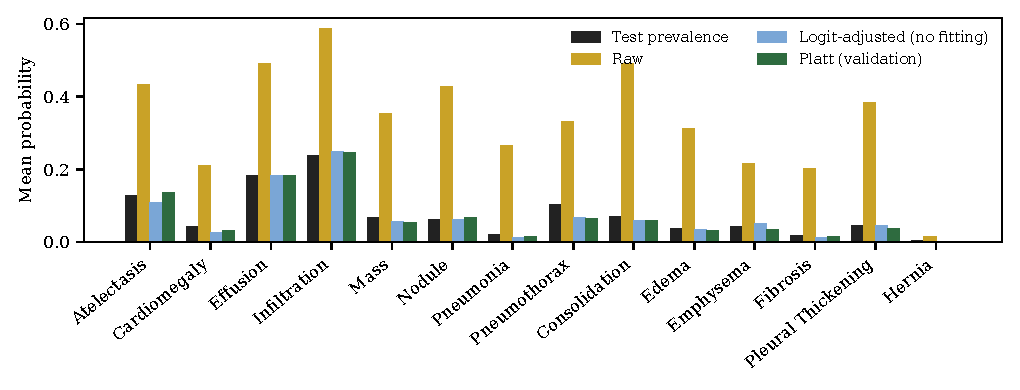
\includegraphics[width=\linewidth]{calibration.pdf}
\caption{Mean predicted probability per label on the test split for DenseNet121 seed 2: raw, after subtracting $\log w_k$ (no fitting), and after Platt scaling fitted on the validation split, against the test prevalence.}
\label{fig:calibration}
\end{figure}

\begin{table}[t]
\centering
\caption{Calibration on the test split, averaged over 14 labels. AUROC is unchanged by both corrections because they are monotonic per label.}
\label{tab:calibration}
\begin{tabular}{lcccccc}
\toprule
& \multicolumn{3}{c}{Mean ECE} & \multicolumn{3}{c}{Mean Brier score} \\
\cmidrule(lr){2-4}\cmidrule(lr){5-7}
Model & Raw & Logit adj. & Platt & Raw & Logit adj. & Platt \\
\midrule
DenseNet121, seed 1 & 0.276 & 0.018 & 0.011 & 0.185 & 0.059 & 0.058 \\
DenseNet121, seed 2 & 0.261 & 0.018 & 0.011 & 0.174 & 0.059 & 0.058 \\
EfficientNet-B0 & 0.291 & 0.016 & 0.011 & 0.195 & 0.059 & 0.059 \\
\bottomrule
\end{tabular}
\end{table}

Raw probabilities are far too high for every label (Figure~\ref{fig:calibration}): the mean predicted probability is 2.3 to 16 times the test prevalence across the three runs (largest for hernia), and mean ECE is 0.26 to 0.29 (Table~\ref{tab:calibration}). For consolidation, the model predicts 0.49 on average while 7\% of test images have the label.

Subtracting $\log w_k$ from the logits removes most of this error without using any validation data: mean ECE falls to 0.016--0.018 and mean Brier score from 0.17--0.20 to 0.059. Platt scaling fitted on 8,805 validation images does slightly better (ECE 0.011, Brier 0.058 to 0.059). The fitted Platt intercepts follow the class-weight offsets closely (correlation between $b_k$ and $-\log w_k$: 0.95), and most fitted slopes are below one (0.59 to 1.28), indicating that the remaining error is mainly over-confidence, which the fixed offset cannot correct. In practice, the closed-form adjustment is a sensible default when no held-out data are available, and a validation-fitted correction is still worth its small cost.

\subsection{Prevalence shift limits both corrections}
\label{sec:shift}

The official ChestX-ray14 test split is not a random sample of patients: 62\% of its images have at least one finding, against 43\% in our validation split, and every label is more common in test (1.1 to 3.4 times; pneumothorax 10.4\% against 3.0\%). Both corrections were derived from data with lower prevalence, so they under-predict on the test set where the shift is largest; across labels, the larger the increase in prevalence, the larger the relative under-prediction after Platt scaling (correlation -0.71). Pneumothorax is the clearest case: after Platt scaling its mean calibrated probability is 0.065 against a prevalence of 0.104, and its ECE (0.041) is the worst of all labels; the logit-adjusted model shows the same pattern (ECE 0.046). Calibration is therefore a property of a model \emph{and} a population. A site that adopts such a model would need to recalibrate on its own patients, for example by re-estimating label priors~\cite{saerens2002adjusting}.

\subsection{Referral of uncertain images}

A common safety idea is to let the model keep its most confident images and refer the rest. Ranking images by mean binary entropy and keeping the 50\% with the lowest entropy raises DenseNet121 seed 2 from 0.803 to 0.822 mean AUROC with raw probabilities, but only to 0.807 with calibrated probabilities; for EfficientNet-B0 the calibrated gain is close to zero. Calibrated entropy reflects how common a finding is more than how hard an image is, so it is a weak referral signal on its own.

\subsection{A misleading subgroup result}
\label{sec:subgroups}

\begin{table}[t]
\centering
\caption{Mean test AUROC by subgroup for the three DenseNet121 seeds (42 / 1 / 2), over all 14 labels and over labels with at least 10 positives in the subgroup.}
\label{tab:subgroups}
\begin{tabular}{lrll}
\toprule
Subgroup & Images & All labels & Labels with $\geq$10 positives \\
\midrule
Men & 14,882 & 0.799 / 0.798 / 0.801 & 0.799 / 0.798 / 0.801 \\
Women & 10,714 & 0.804 / 0.803 / 0.804 & 0.804 / 0.803 / 0.804 \\
Age under 40 & 8,290 & 0.764 / 0.767 / 0.796 & 0.802 / 0.804 / 0.804 (no hernia) \\
Age 40--59 & 11,224 & 0.801 / 0.797 / 0.801 & 0.801 / 0.797 / 0.801 \\
Age 60--100 & 6,078 & 0.788 / 0.788 / 0.789 & 0.788 / 0.788 / 0.789 \\
\bottomrule
\end{tabular}
\end{table}

\begin{figure}[t]
\centering
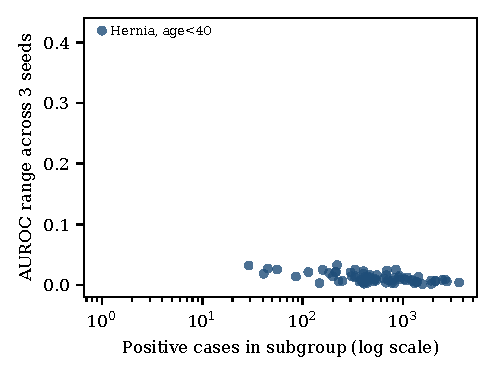
\includegraphics[width=0.55\linewidth]{subgroup_noise.pdf}
\caption{Range of per-label AUROC across the three DenseNet121 seeds against the number of positive cases in each subgroup--label cell. Cells with very few positives produce AUROC values that change wildly between seeds.}
\label{fig:noise}
\end{figure}

Our first subgroup analysis suggested that the model was worse and unstable for patients under 40: mean AUROC over 14 labels was 0.767 and 0.796 for two DenseNet121 seeds and 0.741 for EfficientNet-B0. Counting positives explained it. The 8,290 test images of patients under 40 contain exactly one hernia case, so the hernia AUROC in that group is decided by where one image ranks (from 0.14 to 0.69 across the four runs), and that single number moved the 14-label mean. Restricting the mean to labels with at least 10 positives in the group, patients under 40 score the same as the rest of the test set (Table~\ref{tab:subgroups}). Men and women differ by at most 0.006, and the oldest band is lowest by about 0.01. Figure~\ref{fig:noise} shows how isolated the problem is: across all subgroup--label cells, the AUROC range between the three DenseNet121 seeds is at most 0.033 whenever a cell has 29 or more positives, but 0.42 for the cell with one positive. Subgroup tables should report positive counts per cell and either exclude or pool sparse cells.

\subsection{Deployment check}

We exported DenseNet121 seed 2 to ONNX with two outputs, raw probabilities and class activation maps (for global average pooling followed by one linear layer these equal Grad-CAM~\cite{selvaraju2017gradcam} up to a constant), and built a static web app that runs it in the browser with ONNX Runtime Web and applies the validation-fitted calibration. A canvas resize differs from the Pillow resize used in training and changed probabilities by up to 4 percentage points; reimplementing Pillow's antialiased bilinear filter in JavaScript (maximum difference of one grey level) brought the browser outputs within 0.2 percentage points of the Python reference on three test images.

\section{Limitations}

All images come from one hospital, labels were mined from report text and are known to be noisy~\cite{oakdenrayner2020exploring}, and we use $224\times224$ input with flips only, so absolute AUROC is below strong published results. Only DenseNet121 has several seeds. The logit adjustment assumes that training converged to the weighted-loss optimum; it worked well here but is not guaranteed for other set-ups. We did not annotate chest drains, so we cannot test the drain shortcut for pneumothorax~\cite{oakdenrayner2020hidden}, although its heatmaps spread over both lungs rather than the pleural edge. The models are research artefacts, not medical devices.

\section{Conclusion}

For a class-weighted multi-label chest X-ray classifier, mean AUROC was stable across seeds, but the probabilities were badly miscalibrated by an amount that the class weights predict. Subtracting the log weights is a free first fix; fitting on held-out patients is better; and neither holds when label prevalence shifts. Subgroup claims need positive counts next to them. We recommend reporting calibration alongside AUROC, stating whether class weights were used and how they were corrected, and publishing subgroup tables with their counts.

\section*{Code and data availability}
Code, training notebooks, saved predictions, analysis scripts and tests: \url{https://github.com/MHKhan50/lung-disease-classification} (archived at \href{https://doi.org/10.5281/zenodo.23065563}{doi:10.5281/zenodo.23065563}). Browser demo: \url{https://huggingface.co/spaces/MHkhan50/chest-xray-14-findings}. ChestX-ray14 is provided by the NIH Clinical Center.

\bibliographystyle{unsrtnat}
\bibliography{references}

\end{document}
